\documentclass[0-protokol.tex]{subfiles}
\begin{document}

Pomocí digitálního konduktometru byla změřena měrná elektrická vodivost destilované vody při teplotě $\SI{21}{\celsius}$
$$ \sigma_{H_2O} = \SI{1.05 \pm 0.01}{\micro\siemens\per\centi\metre}.$$
Chyba hodnoty byla určena podle chyby přístroje na $\SI{0.5}{\percent}$ z naměřené hodnoty.

Pomocí pipety byly připraveny vodní roztoky kyseliny chlorovodíkové, sloužící jako silný elektrolyt, a octové jakožto slabý elektrolyt o celkových objemech $\SI{100}{ml}$. Pomocí konduktometru byla čtyřikrát změřena hodnota měrné vodivosti roztoku \textit{HCl}, výsledek je uveden v tabulce \ref{tab:chyba}. Pomocí vzorce \eqref{eq:chyba} byla spočítaná statistická chyba měření $s_\sigma = \SI{0.97}{\micro\siemens\per\centi\metre} \doteq \SI{1}{\micro\siemens\per\centi\metre}$. S touto zaokrouhlenou hodnotou je dále nakládáno jako s statistickou chybou měření všech dalších hodnot. Chyba pipety je považována za součást této chyby, chybu konduktometru je především u koncentrovanějších roztoků $HCl$ přičíst podle \eqref{eq:chyba_soucet}.

\begin{table}[H] 
\centering
\setlength{\tabcolsep}{10pt}
\begin{tabular}{
    l
    S[table-format=3.1]
    S[table-format=3.1]
    S[table-format=3.1]
    S[table-format=3.1]
}                                                                                                \toprule
měření                                                                     & {1}   & {2}   & {3}  & {4}   \\ \midrule
$\sigma_{\textit{HCl}}^{\SI{2}{ml}}\, [\si{\micro\siemens\per\centi\metre}]$ & 109.9 & 111.8 & 112  & 110.8 \\
$t\, [\si{\celsius}]$                                                        & 20.5  & 20.2  & 20.3 & 20.7  \\ \bottomrule
\end{tabular}
\caption{Čtyři měření měrné vodivosti roztoku \SI{2}{ml} \textit{HCl}}
\label{tab:chyba}
\end{table}

Následující tabulka shrnuje naměřené hodnoty měrných vodivostí roztoků kyseliny chlorovodíkové a octové spolu s přepočtem objemových zlomků rozpuštěných látek na molární koncentrace a jejich molární konduktivity.

\begin{table}[H] 
\centering
\setlength{\tabcolsep}{10pt}
\begin{tabular}{
    l
    c
    c
    c
    c
    c
    c
} \toprule
$V_0\, [\si{ml}]$                                               & 1      & 2      & 4      & 6      & 8      & 10     \\ \midrule
$c_{M_{CH_3COOH}}\, [\si{\mole\per\cubic\metre}]$               & 0,1    & 0,2    & 0,4    & 0,6    & 0,8    & 1      \\
$\sigma_{CH_3COOH}\, [\si{\micro\siemens\per\centi\metre}]$     & 38,5   & 53,3   & 77,9   & 97,9   & 112,5  & 126,2  \\
$s_{\sigma_{CH_3COOH}}\, [\si{\micro\siemens\per\centi\metre}]$ & 1,0    & 1,0    & 1,1    & 1,1    & 1,1    & 1,2    \\
$\Lambda_{CH_3COOH} [\si{\siemens\metre\squared\per\mole}]$     & 0.0385 & 0.0266 & 0.0195 & 0.0163 & 0.0141 & 0.0126 \\
$s_{\Lambda_{CH_3COOH}} [\si{\siemens\metre\squared\per\mole}]$ & 0.0010 & 0.0005 & 0.0003 & 0.0002 & 0.0001 & 0.0001 \\ \midrule[0.3pt]
$c_{M_{HCl}}\, [\si{\mole\per\cubic\metre}]$                    & 0,5    & 1      & 2      & 3      & 4      & 5      \\
$\sigma_{HCl}\, [\si{\micro\siemens\per\centi\metre}]$          & 54,1   & 109,9  & 216    & 332    & 436    & 549    \\
$s_{\sigma_{HCl}}\, [\si{\micro\siemens\per\centi\metre}]$      & 1      & 1,1    & 1,4    & 1,9    & 2,3    & 2,9    \\
$\Lambda_{HCl} [\si{\siemens\metre\squared\per\mole}]$          & 0.0108 & 0.0110 & 0.0108 & 0.0111 & 0.0109 & 0.0110 \\
$s_{\Lambda_{HCl}} [\si{\siemens\metre\squared\per\mole}]$      & 0.0002 & 0.0001 & 0.0001 & 0.0001 & 0.0001 & 0.0001 \\ \bottomrule
\end{tabular}
\caption{Tabulka naměřených a spočtených hodnot pro silný a slabý elektrolyt}
\label{tab:koncentrace}
\end{table}

Následující grafy znázorňují průběh závislosti $\Lambda$ na $\sqrt{c_M}$.

\begin{figure}[H]
\centering
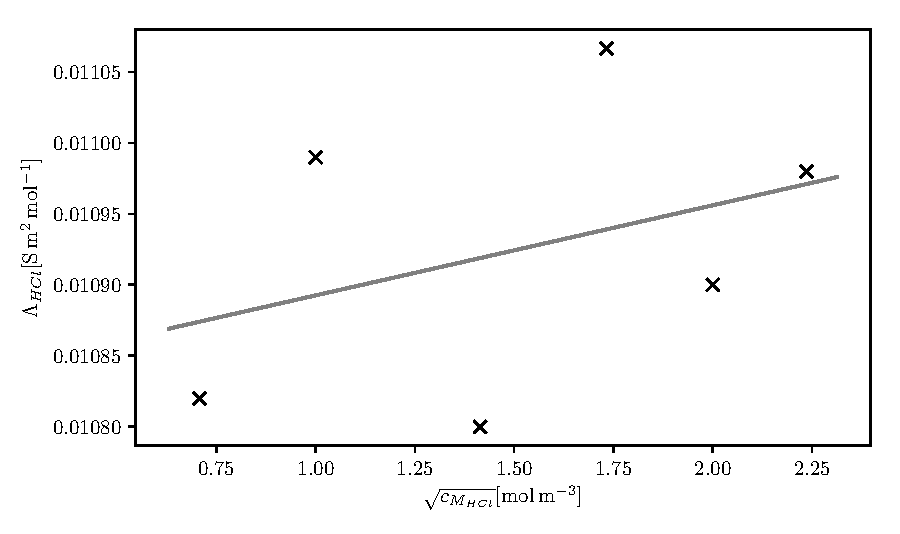
\includegraphics[]{silny}
\caption{Závislost molární konduktivity roztoku kyseliny chlorovodíkové na odmocnině z molární koncentrace}
\label{fig:silny}
\end{figure}

\begin{figure}[H]
\centering
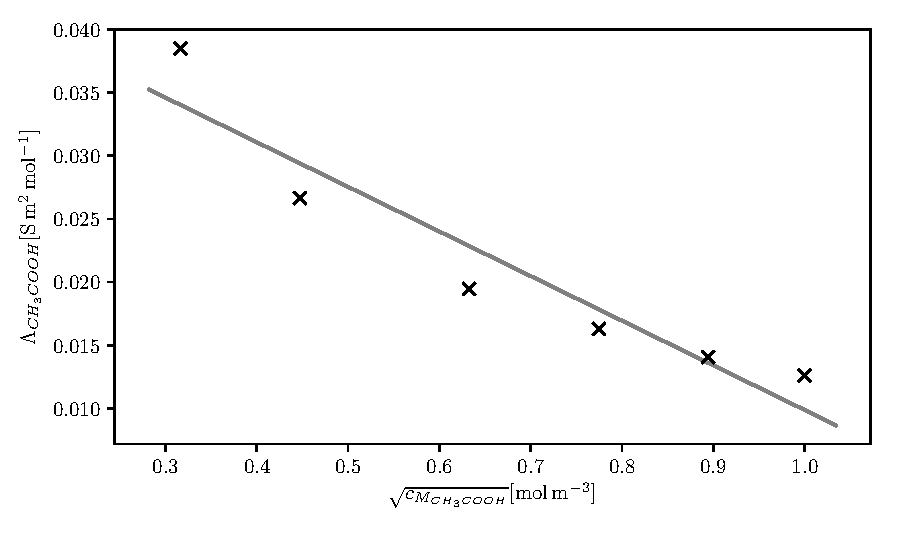
\includegraphics[]{slaby}
\caption{Závislost molární konduktivity roztoku kyseliny octové na odmocnině z molární koncentrace}
\label{fig:slaby}
\end{figure}

Z lineárních regresí byly odečteny hodnoty 
$$ \Lambda_{0_{HCl}} = \SI{0.01083 \pm 0.00020}{\siemens\metre\squared\per\mole},$$
$$ \Lambda_{0_{CH_3COOH}} = \SI{0.045 \pm 0.004}{\siemens\metre\squared\per\mole}. $$

\end{document}
